
\chapter{APPLYING THE NEW SIMILARITY THEORY TO THE SHELL \\ MODEL DATA} \label{ch: before the theory}

In the theoretical analysis in Chapter \ref{ch:a new theory}, we found the similarity formulas for the inertial range in terms of four constants $\beta$, $n_0$, $a$, $C_3$ (five if $\zeta_3$ is included) .  While this may seem like many constants to determine, one should keep in mind that two constants are unavoidable.  There has to be a characteristic length, $\ell_0$, equivalently, $n_0$ performs this function.  Also, there has to be a constant characterizing the forcing rate, (related to the dissipation rate because this system is in equilibrium).  $C_3$ performs this role.  $\beta$ and $a$ came about through the functional equation (\ref{eq: ant R1} and \ref{eq: ant R2}).  The theory does not provide values for these constants other than $0<\beta<3$ and $a<0$.

In this chapter, we will use the data form the Sabra model to find $\beta$ and $a$.  Because the GOY model data does not meet our standards for the power law requirement, it cannot be expected to follow the theory. First, we show how the power laws can be plotted so as to reveal $n_0$ and $C_3$.  This is theoretically possible because we have found a universal expression for the coefficients $C_p$.  The technique is to introduce rescaled structure functions. Second, we examine the data to see if the horizontal stretching fits the theoretical expression $(\ln \ell_0 - \ln \ell)^{1/\beta}$ or equivalently a power law in $n - n_0$.  Likewise, we can check if the horizontal and vertical shifts are linear functions of $n$ as predicted by the theory.  Finally, we can extract $\beta$ and $a$ from the data.

\vspace{2in}

\section{Determination of $n_0$ and $C_3$ via Rescaled Structure Functions}

When we previously defined structure functions, we neglected to include an intrinsic length scale.  The intrinsic scale plays an important role in regard to the scaling coefficients, $\tilde{C}_p$. Without an intrinsic scale, the coefficients cannot be described in universal terms.  The reason is that any factor of the form $2^{n_1\zeta_p}$ can be attached to the coefficient.  In other words, we can write
\begin{eqnarray}
    S_p(n) & = & \tilde{C}_p2^{-n\zeta_p} \nonumber \\
    & = & \tilde{C}_p2^{n_1\zeta_p}2^{-\zeta(n-n_1)}
\end{eqnarray}
and redefine the coefficient as $\tilde{C}_p2^{n_1\zeta_p}$.  Only when we can fix $n_1$ at some preferred value, like an intrinsic scale $n_0$, can we talk about universal coefficients. The theoretical formulas from the previous chapter \cite{Melander2007} state
\begin{equation}
    S_{p}(\ell) = C_{p}\left(\frac{\ell}{\ell_{0}}\right)^{\zeta_{p}}.
\end{equation}
Using $\ell = 2\pi/k$, where $k = k_{0}2^{n}$, we can translate to shell notation.  Hence, we replace $\ell$ with $2\pi/(k_{0}2^{n})$, we get
\begin{eqnarray}
    S_{p}(n) & = & C_{p}\left(\frac{2\pi/(k_{0}2^{n})}{2\pi/(k_{0}2^{n_{0}})}\right)^{\zeta_{p}} \nonumber \\
    & = & C_{p}\left(\frac{2^{n_{0}}}{2^{n}}\right)^{\zeta_{p}} \nonumber \\
    & = & C_{p}2^{-\zeta_{p}(n-n_{0})} . \label{eq: new sfp}
\end{eqnarray}

To rescale the structure functions, we must know $C_{p}$.  Again, we use the theoretical formula for the universal coefficients found in \cite{Melander2007},
\begin{equation}
    C_{p} = \frac{2}{p+2}\left(\frac{5C_{3}}{2}\right)^{p/3}. \label{eq: theoretical cp}
\end{equation}
Thus,  (\ref{eq: new sfp}) reads
\begin{equation}
    S_{p}(n)  =  \frac{2}{p+2}\left(\frac{5C_{3}}{2}\right)^{p/3}2^{-\zeta_{p}(n-n_{0})} . \label{eq: sfp with theoretical cp}
\end{equation}
Next, we will take the natural logarithm of both sides:
\begin{equation}
    \ln\left(S_{p}(n)\right) = \ln\left[\frac{2}{p+2}\left(\frac{5C_{3}}{2}\right)^{p/3}2^{-\zeta_{p}(n-n_{0})}\right]
\end{equation}
or
\begin{equation}
    \ln\left(S_{p}(n)\right) = \ln\left(\frac{2}{p+2}\right) + \frac{p}{3}\ln\left(\frac{5C_{3}}{2}\right) -\zeta_{p}(n-n_{0})\ln2
\end{equation}
then
\begin{equation}
    \ln\left(\frac{S_{p}(n)(p+2)}{2}\right) = \frac{p}{3}\ln\left(\frac{5C_{3}}{2}\right) -\zeta_{p}(n-n_{0})\ln2.
\end{equation}
Our final step is to move $p$ to the left hand side
\begin{equation}
    \frac{1}{p}\ln\left(\frac{S_{p}(n)(p+2)}{2}\right) = \frac{1}{3}\ln\left(\frac{5C_{3}}{2}\right) -\frac{1}{p}\zeta_{p}(n-n_{0})\ln2 .\label{eq: log similarity formula 2}
\end{equation}
The left hand side is the data we plot. Whereas, the right hand side is the theoretical expression. When plotted against $n$, the theoretical expression calls for $1/p\ln\left(\frac{S_{p}(n)(p+2)}{2}\right)$ to form a set of straight lines (one for each $p$), with a single point in common, namely ($n_0$, $1/3\ln\left(5C_3/2\right)$.

It is for this reason we have introduced the rescaled structure functions.  This is shown in Figure \ref{fig: at focus}. Note, in the absence of anomalous scaling, i.e. $\zeta_p = p/3$, (\ref{eq: log similarity formula 2}) produces the same straight line for all $p$.  Thus, the spread of the lines in Figure \ref{fig: at focus} is a signature of anomalous scaling.

The theoretical expression is, of course, only valid when $n$ is in the inertial range.  By fitting straight lines to the power laws in the inertial range, as is done in Figure \ref{fig: at focus}, we extrapolate to find the focusing point for all the lines.  In fact, we observe that the lines have an approximate common point of intersection.  The focusing confirms the theoretical expression for the scaling coefficients in (\ref{eq: theoretical cp}). If (\ref{eq: theoretical cp}) did not apply the lines would not intersect at the same point.

The common point of intersection forms the virtual origin for the inertial range.  That is, the scaling laws cannot be continued to larger scales (smaller $n$). In fact, $n_0$ is the smallest $n$ for $S_{p}(n)$ in (\ref{eq: sfp with theoretical cp}) that corresponds to a pdf.

Figure \ref{fig: at focus} is significant for many reasons.  Not only does it determine an intrinsic length scale  for the inertial range, and confirm the theoretical coefficient formula (\ref{eq: theoretical cp}), it also shows that all $S_{p}(n)$ can be computed from $S_{p}(\tilde{n})$ and the virtual origin, where $\tilde{n}$ represents a single shell located inside the inertial range.  This fact alone shows that the inertial range is self-similar.  If we know all $S_{p}(\tilde{n})$ for some value of $\tilde{n}$, then the radial profile can be determined through an inverse Mellin transform. The similarity implied by Figure \ref{fig: at focus} then allows us to obtain the radial profile for all inertial range shells.

\begin{figure}[!hpt]
    \begin{center}
    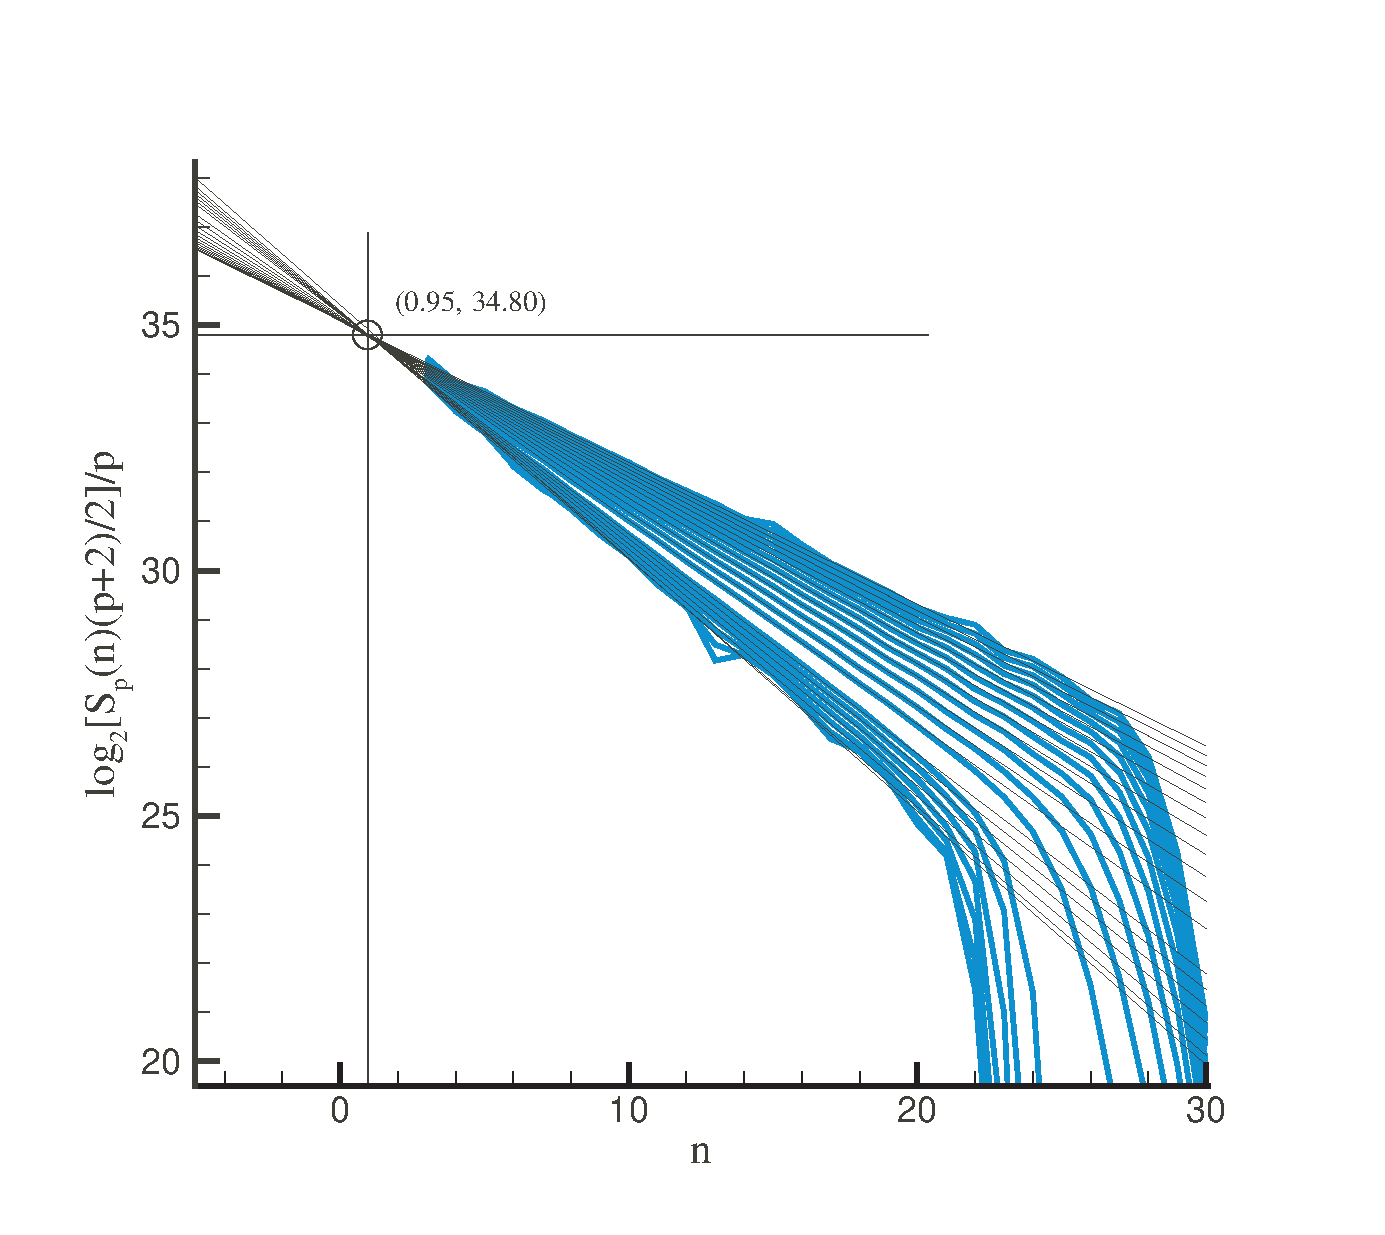
\includegraphics[width=4in]{at_focus.eps}
    \end{center}
    \caption{Rescaled structure function of Run 9 from Table \ref{table: app Sabra table} (Sabra). The functions can be formed because we have found universal coefficients.  $p = [-1.75, -1.5, \cdots, -0.5, -0.25, 0, 0.5, 1.0, \cdots, 11.5, 12.0]$} \label{fig: at focus}
\end{figure}

\subsection{The Limit of $p \rightarrow 0$}

Figure \ref{fig: at epsilon}.a show where $p = 0$ would be in the graph of rescaled structure functions.  This is due to (\ref{eq: log similarity formula 2}) involving a division by zero for $p = 0$.  Nonetheless, we can define a rescaled structure function for $p = 0$ through a limiting process.  Figure \ref{fig: at epsilon}.b clearly suggest that there are no problems for small $p$.  On the right hand side of (\ref{eq: log similarity formula 2}) it is the factor $\zeta_p/p$ that causes the problem.  Since $\zeta_0 = 0$, L'Hopitals rule can be applied.  In fact, the singularity at $p = 0$ is removable. We implement L'Hopitals rule for the data by means of a difference quotient:
\begin{equation}
    \lim_{p \rightarrow 0}\tilde{S}_p = \lim_{p \rightarrow 0}\frac{\tilde{S}_p - \tilde{S}_{-p}}{2p}.
\end{equation}
where
\begin{equation}
    \tilde{S}_p = \frac{1}{p}\ln\left(\frac{S_{p}(n)(p+2)}{2}\right).
\end{equation}

\begin{figure}[!hpt]
    \hspace{1.5in}{\centering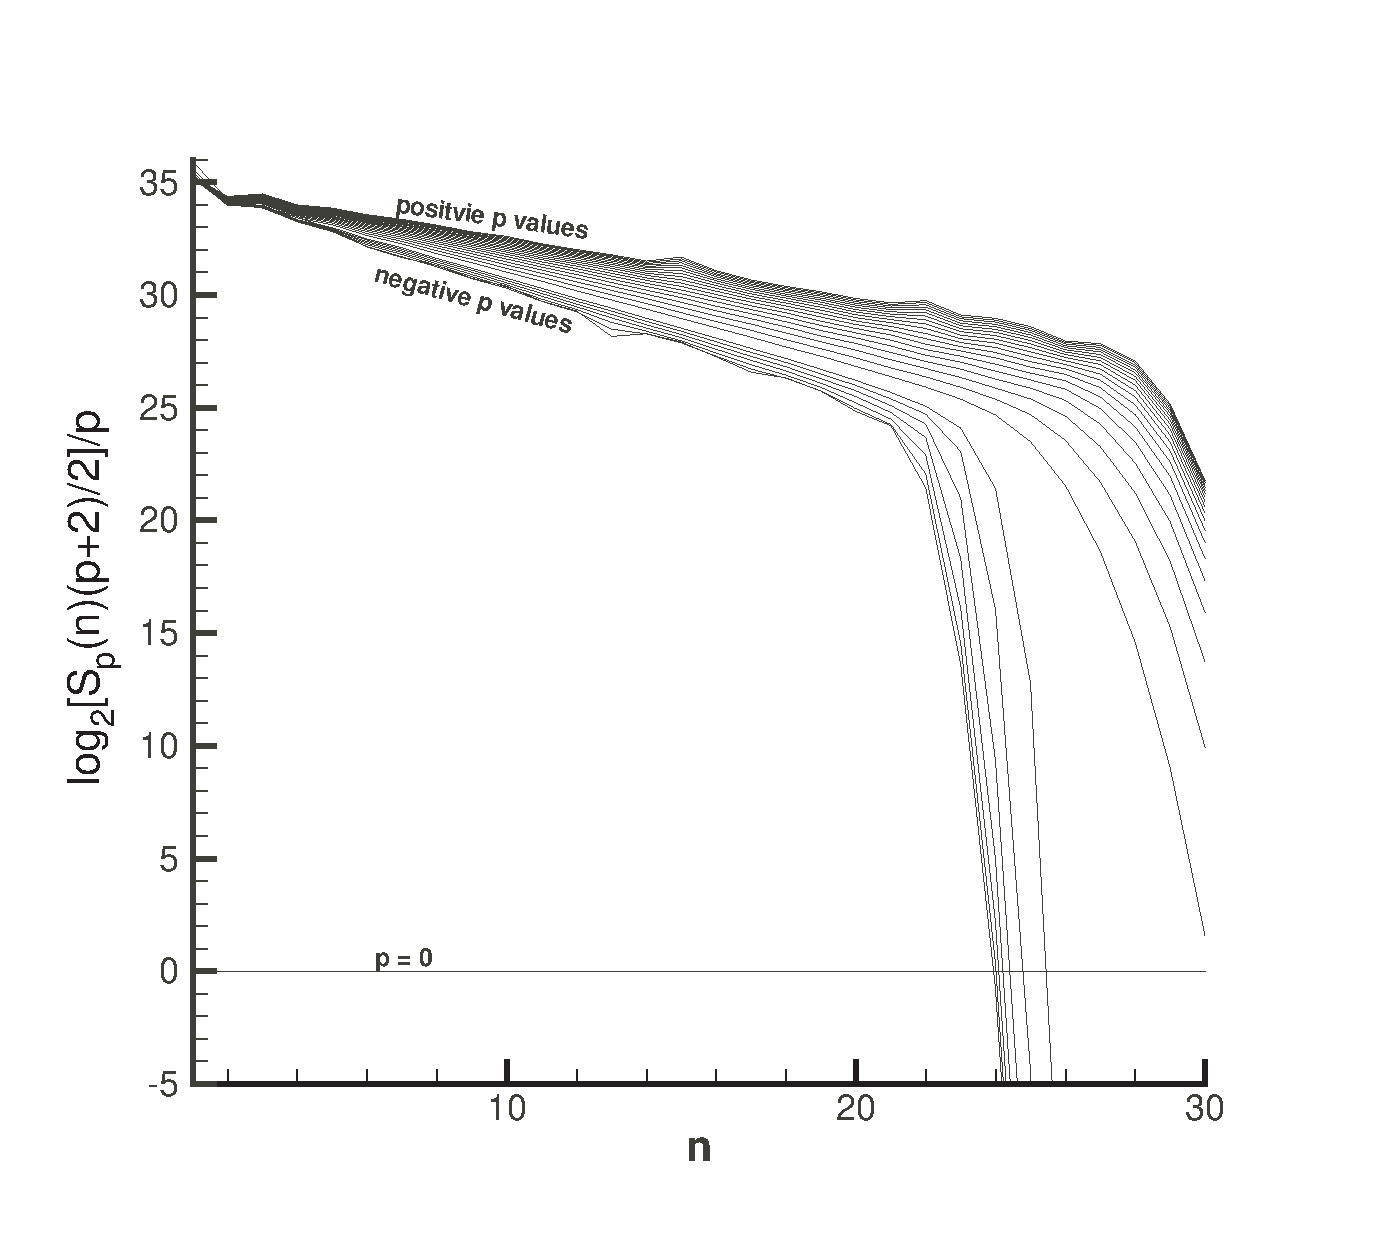
\includegraphics[width=4in]{tt_epsilon_with_0.eps}}\\

    \hspace{1.5in}{\centering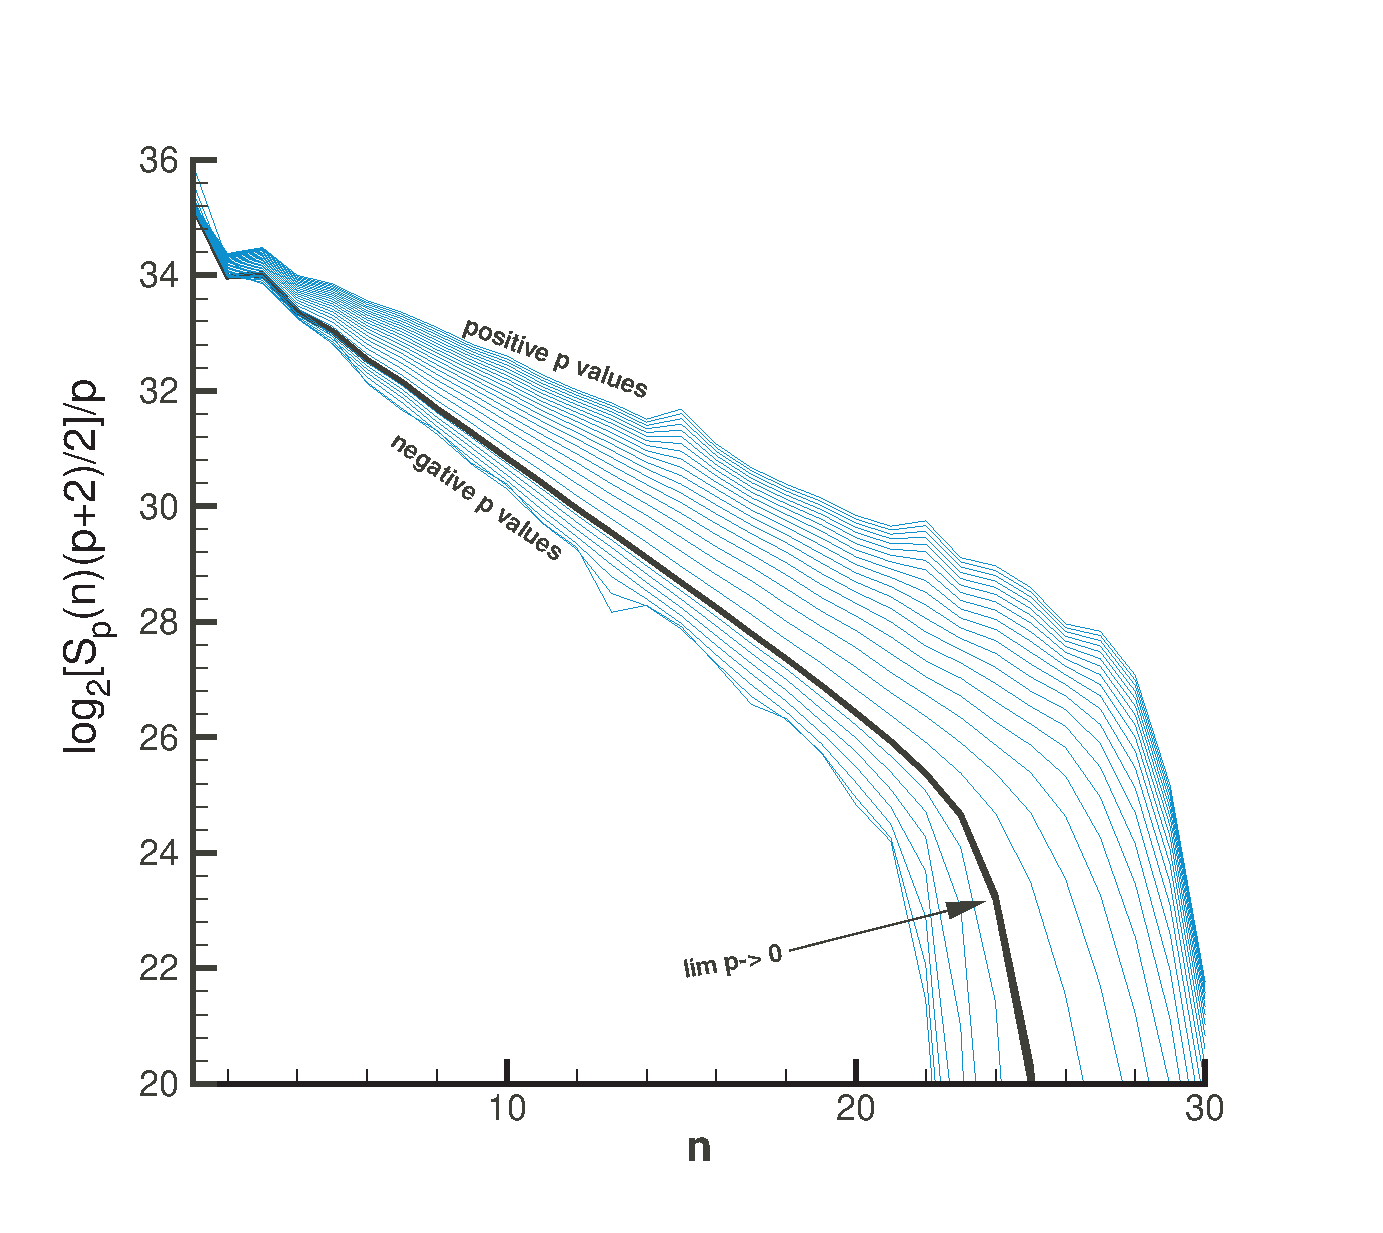
\includegraphics[width=4in]{tt_epsilon.eps}}
    \caption{Rescaled structure function of Run 9 from Table \ref{table: app Sabra table} (a) with $p = 0$ included. Note the gap between the negative and positive $p$ values. (b) as $p \rightarrow 0$  where $0.1 \geq p \geq 0.01$. Clearly a limit exists.} \label{fig: at epsilon}
\end{figure}

%\begin{equation}
%    \zeta_{p} - \frac{p}{3} = \frac{a}{3\beta(\beta-1)}\left[3(p+2)^{\beta} + (2^{\beta} - 5^{\beta})(p+2) + 2 \times5^{\beta} - 5\times2^{\beta} \right] \label{eq: Zetap}.
%\end{equation}

\vspace{2in}

\section{Graphically Measured Collapse}

Figure \ref{fig: all plots} show log-log plots of the radial profile $P_0(r;n)$ for $n$ ranging from 3 to 20.  As described in Chapter \ref{ch:self similarity of the joint pdf}, these graphs can be made to collapse by a similarity transformation.  Specifically, rigid horizontal shifts together with linear horizontal stretching.  Both shifts and stretching can be measured.  The process is as follows.  We first select one reference shell in the middle of the inertial range.  Let that be $n=12$.  The graphical objects corresponding to each of the other shells are then shifted rigidly and stretched horizontally so that the graphs match that of $P_0(r;12)$ as shown in Figures \ref{fig: s4and5with12} through \ref{fig: s19and20with12}.  Because the axes from Figure \ref{fig: all plots} are attached to $P_0(r;n)$ we can readily identify the vertical shift.  It is listed in Table \ref{table: measurements}.  We can also identify matching abscissa on the fixed and transformed scale.  The horizontal bars in Figure \ref{fig: s4and5with12} through \ref{fig: s19and20with12} are included for this purpose.  The corresponding abscissa pairs are listed in Table \ref{table: measurements}.  Since the transformation is linear only two values are needed for each $n$.  From these values we calculate the horizontal stretching factor $A$ and shift $B$, i.e.
\begin{equation}
	x_{stretched} = Ax_{f} + B
\end{equation}
Say $a$ and $b$ are two points on the fixed axis corresponding to $c$ and $d$ on the stretched axis, then
\begin{eqnarray}
	c & = & Aa + B \\
	d & = & Ab + B.
\end{eqnarray}
So that,
\begin{eqnarray}
	A & = & \frac{a-b}{c-d} \\
	B & = & \frac{bc-ad}{b-a}.
\end{eqnarray}
Figure \ref{fig: shifts} shows the vertical and horizontal shifts as functions of $n$.  We observe that both are linear functions of $n$ as called for by the theory.  The scatter around the regression line is in part due to the matching of the graphical objects being done manually.  The theory does provide analytical formulas to do a computational collapse.  However, the data we obtained contained too much statistical noise.  Therefore, we were not able to use the analytical formulas.  The vertical shift is also shown.  It forms a straight line on log-log scales.  Consequently, the stretching is a power law in $(n-n_0)$ just as predicted by the theory.  The slope is $1/\beta$ and we obtain $\beta = 1.23$ from the regression line.

\begin{table}[!htp]
    \begin{center}
    \caption{Measurements for scaling individual radial profiles.  Shell 12 is selected as the radial profile to be scaled to.  The fixed scale refers to the Shell 12 axis. The first pair of fixed and stretched scales refers to the initial alignment of the horizontal axis.  The second pair refers to the terminal alignment of the horizontal axis.}
    \begin{tabular}{||c|c|c|c|c|c||} \hline	
        \multicolumn{6}{|c|}{\emph{Measurements for Graphical Collapse}} \\ \hline \hline
        Shell & Fixed Scale & Stretched Scale & Fixed Scale & Stretched Scale & Vertical Shift \\
        \hline
        \hline
        3   &   15   &   22.2    &   21.1    &   24&     7\\
        4   &   16.2 &   22    &   22.1    &   24  &      6.2\\
        5   &   15.6 &   21    &   23.1    &   24  &      5.8\\
        6   &   16   &   21      &   22.8    &   24&      5.6\\
        7   &   14.8 &   19    &   23.2    &   24  &   3.7\\
        8   &   15.8 &   19    &   23.3    &   24  &   3.2\\
        9   &   15.6 &   18    &   23.5    &   24  &   1.8\\
        10   &   15.7&   17    &   23.6    &   24  &   1.2\\
        11   &   15.2&   16    &   23.8    &   24  &   0.8\\
        13   &   15.5&   15    &   24.3    &   24  &   -0.7\\
        14   &   17  &   15.7    &   24    &   23.6  &   -1.6\\
        15   &   17  &   15.2    &   24    &   24.3  &   -2.4\\
        16   &   18  &   15.6    &   24    &   23.3  &   -2.8\\
        17   &   18  &   15.2    &   24    &   23.1  &   -3.9\\
        18   &   19  &   16      &   24    &   22.8  &   -4.3\\
        19   &   19  &   15.1    &   24    &   22.7  &   -5.8\\
        20   &   20  &   16.1    &   24    &   22.6  &   -6.5\\
        \hline
        \hline
    \end{tabular}
    \end{center}
    \label{table: measurements}
\end{table}


\begin{figure}[!hpt]
    \begin{center}
     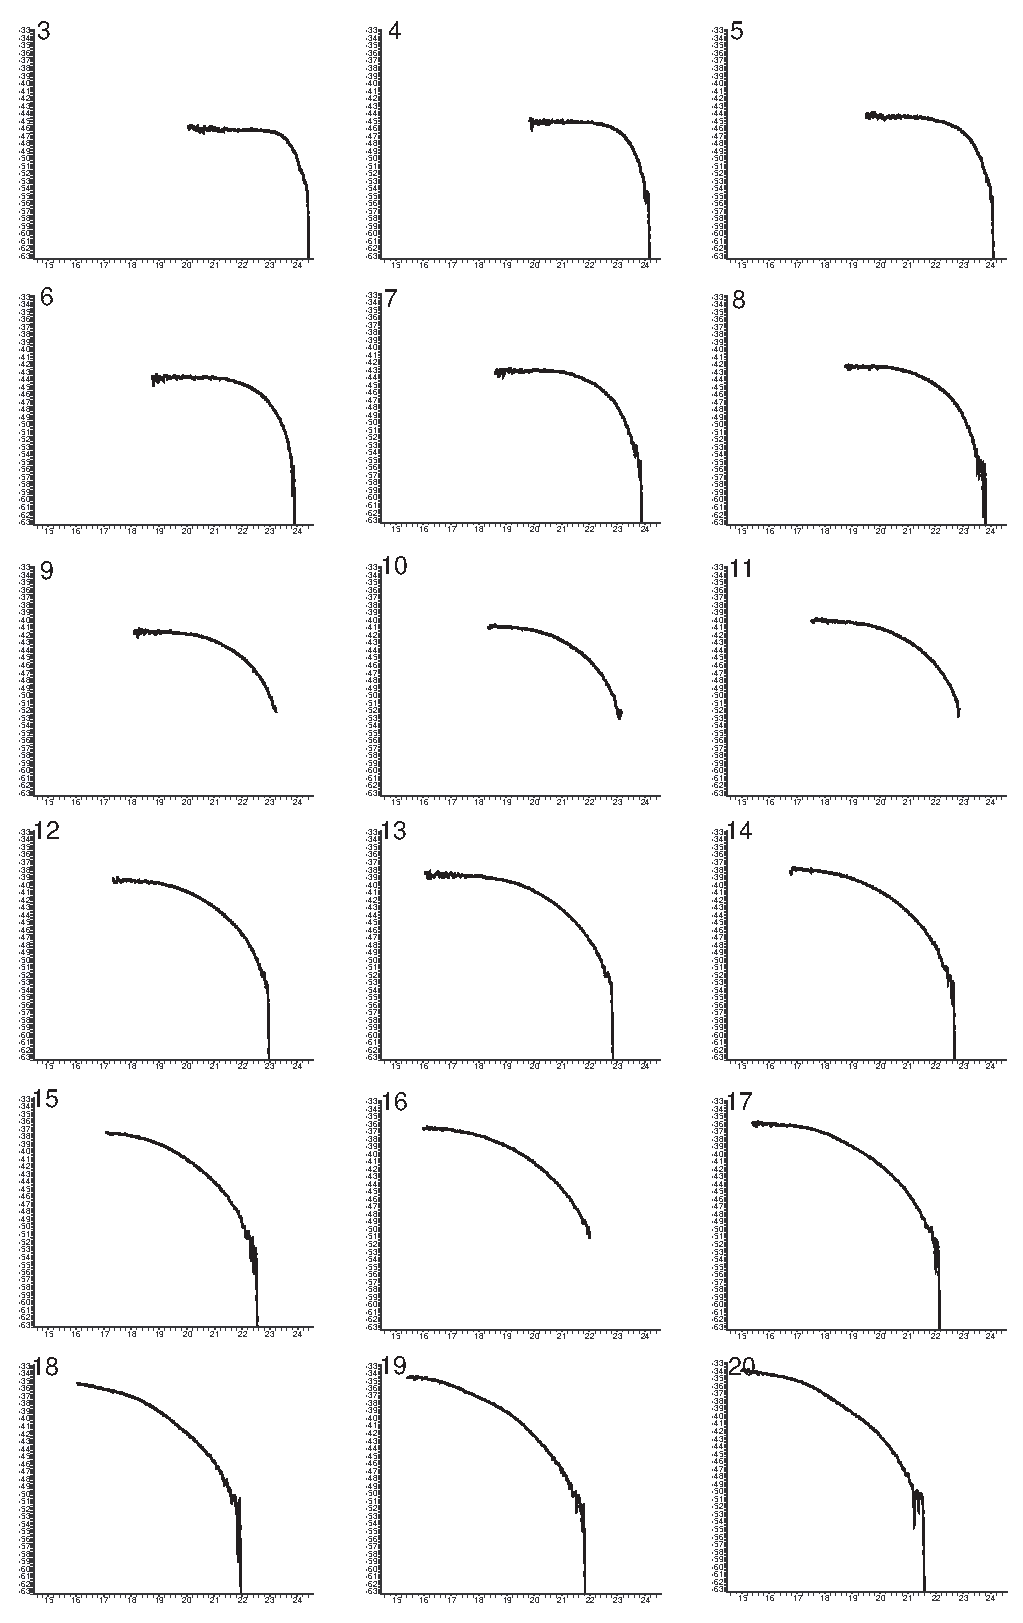
\includegraphics[width=4in]{allplots.eps}
     \end{center}
  \caption{Individual plots of each of the radial profiles that have a similar curve. The radial profiles $P_0(r;n)$ plotted on log-log scales for $3\leq n \leq 20$ for Sabra Run 9.} \label{fig: all plots}
\end{figure}

\begin{comment}
\begin{figure}[!hpt]
    \begin{center}
     \includegraphics[width=4in]{s4and5with12.eps}
     \end{center}
  \caption{(a) Collapse of $P_0(r;4)$ onto $P_0(r;12)$ using horizontal and vertical shift s together with horizontal stretching.  The vertical bars correspond to the numbers in Table (b) collapse of $P_0(r;5)$ onto $P_0(r;12)$.} \label{fig: s4and5with12}
\end{figure}

\begin{figure}[!hpt]
    \begin{center}
     \includegraphics[width=4in]{s6and7with12.eps}
     \end{center}
  \caption{(a) Collapse of $P_0(r;6)$ onto $P_0(r;12)$ (b) collapse of $P_0(r;6)$ onto $P_0(r;12)$.} \label{fig: s6and7with12}
\end{figure}

\begin{figure}[!hpt]
    \begin{center}
     \includegraphics[width=4in]{s8and9with12.eps}
     \end{center}
  \caption{(a) Collapse of $P_0(r;8)$ onto $P_0(r;12)$ (b) collapse of $P_0(r;9)$ onto $P_0(r;12)$.} \label{fig: s8and9with12}
\end{figure}

\begin{figure}[!hpt]
    \begin{center}
     \includegraphics[width=4in]{s10and11with12.eps}
     \end{center}
  \caption{(a) Collapse of $P_0(r;10)$ onto $P_0(r;12)$ (b) collapse of $P_0(r;11)$ onto $P_0(r;12)$.} \label{fig: s10and11with12}
\end{figure}

\begin{figure}[!hpt]
    \begin{center}
     \includegraphics[width=4in]{s13and14with12.eps}
     \end{center}
  \caption{(a) Collapse of $P_0(r;13)$ onto $P_0(r;12)$ (b) collapse of $P_0(r;14)$ onto $P_0(r;12)$.} \label{fig: s13and14with12}
\end{figure}

\begin{figure}[!hpt]
    \begin{center}
     \includegraphics[width=4in]{s15and16with12.eps}
     \end{center}
  \caption{(a) Collapse of $P_0(r;15)$ onto $P_0(r;12)$ (b) collapse of $P_0(r;16)$ onto $P_0(r;12)$.} \label{fig: s15and16with12}
\end{figure}

\begin{figure}[!hpt]
    \begin{center}
     \includegraphics[width=4in]{s17and18with12.eps}
     \end{center}
  \caption{(a) Collapse of $P_0(r;17)$ onto $P_0(r;12)$ (b) collapse of $P_0(r;18)$ onto $P_0(r;12)$.} \label{fig: s17and18with12}
\end{figure}

\begin{figure}[!hpt]
    \begin{center}
     \includegraphics[width=4in]{s19and20with12.eps}
     \end{center}
  \caption{(a) Collapse of $P_0(r;19)$ onto $P_0(r;12)$ (b) collapse of $P_0(r;20)$ onto $P_0(r;12)$.} \label{fig: s19and20with12}
\end{figure}

\begin{figure}[!hpt]
    \begin{center}
     \includegraphics[width=2.5in]{shifts.eps}
     \end{center}
  \caption{Graphs of (a) horizontal shift (b) vertical shift and (c) the horizontal stretching factor with regression lines fitted to the data } \label{fig: shifts}
\end{figure}

\section{Extracting the Theoretical Parameters}

In the theoretical formulas, there are four unknown constants that we must find, namely, $\beta$, $a$, $C_3$ and $n_0$. In principle, we also need $\zeta_3$, but we have already found it to be very close to one therefore, we assume $\zeta_3 \equiv 1$ in accordance with the four-fifth's law.  There are several ways to extract the constants from the data. We have seen one way of extracting $n_0$, $C_3$, and $\beta$ in sections 10.1 and 10.2. Now, we discuss two other methods for attaining these parameters.

The first involves divided differences based on the rescaled structure functions.  This method goes through step-by-step eliminating unknowns till $\beta$ is the last unknown available.  Then the method filters back through to give us values for the other unknowns.

The second method uses cumulants.  Through this method, we use ratios and graphs to determine the values.  Using both methods gives us a way to check the accuracy of the values.

\subsection{Divided Differences}

We will use two intermediate variables, $m_{p}$ and $R_{p}$.  Using these variables we will be able to extract $\beta$ which will in turn yield $a$, and we will be able to check the values of $n_{0}$ and $C_{3}$.

To find $m_{p}$, we need to rearrange (\ref{eq: log similarity formula 2}). Moving $\ln (5/2 S_{3})$ from the left and right hand side, we have
\begin{eqnarray}
    m_{p} & \equiv & \frac{3}{p}\ln\left(\frac{S_{p}(n)(p+2)}{2}\right) - \ln \left(\frac{5}{2}S_{3}\right) \nonumber\\
    & = & \ln\left(\frac{5C_{3}}{2}\right) -\frac{3}{p}\zeta_{p}(n-n_{0})\ln2 - \ln \left(\frac{5}{2}S_{3}\right) \nonumber\\
    & = & \ln\left(\frac{5C_{3}}{2}\right) -\frac{3}{p}\zeta_{p}(n-n_{0})\ln2 - \ln\left(\frac{5}{2}C_{3}2^{-\zeta_{3}(n-n_{0})}\right) \nonumber\\
    & = & \ln\left(\frac{5C_{3}}{2}\right) -\frac{3}{p}\zeta_{p}(n-n_{0})\ln2 - \ln\left(\frac{5}{2}C_{3}\right) + \zeta_{3}(n-n_{0}) \ln2 \nonumber\\
    & = & -\frac{3}{p}\zeta_{p}(n-n_{0})\ln2  + \zeta_{3}(n-n_{0}) \ln2
\end{eqnarray}
or, with $\zeta_3 = 1$:
\begin{equation}
    m_p =  \left(1-\frac{3}{p}\zeta_{p}\right)(n-n_{0})\ln2. \label{eq: mp}
\end{equation}
Through this process we have eliminated $C_{3}$ and are left with three unknowns. Note, theoretically $m_3 \equiv 0$.

\begin{figure}[!hpt]
    \begin{center}
    \includegraphics[width=4in]{at_mp_vs_m2.eps}
    \end{center}
    \caption{Plot of $m_p$ vs. $m_2$. Straight lines are superimposed over the different data sets. The data sets are represented by squares.} \label{fig: at mp vs m2}
\end{figure}

The theoretical expression (\ref{eq: mp}) vanishes for $n = n_0$ for all $p$ and is linear in $n - n_0$.  Consequently, $(m_2, m_p)$ constitutes a parameteric representation for a straight line with $(n - n_0)$ as the parameter.  This line passes through (0,0) regardless of the value of $p$.

Figure \ref{fig: at mp vs m2} shows $m_{p}$ vs. $m_{2}$. We substitute in the regression line values we found previously for $\zeta_p$.  Using this figure, the power laws are tested once more.  The straight lines through the points are a clear indication that the power laws do hold.  Note, that all lines meet at $(0,0)$. Thus, the ratio of $m_{p}$ and $m_{2}$ is independent of $n-n_{0}$ in the power law regime, i.e.
\begin{equation}
    \frac{m_{p}}{m_{2}} = \frac{\left(1-\frac{3}{p}\zeta_{p}\right)(n-n_{0})\ln2}{\left(1-\frac{3}{2}\zeta_{2}\right)(n-n_{0})\ln2}.
\end{equation}
This eliminates $n_{0}$ from the equation. We will call the reduced ratio $R_p$, i.e.
\begin{equation}
    R_p =  \frac{\left(1-\frac{3}{p}\zeta_{p}\right)}{\left(1-\frac{3}{2}\zeta_{2}\right)} \label{eq: rp in process}
\end{equation}

Next, we substitute the expressions for $\zeta_{p}$ and $\zeta_{2}$ into (\ref{eq: rp in process}). In doing so, we find that $R_p$ is independent of $a$,
\begin{eqnarray}
     R_{p} & = & \frac{\frac{a}{p\beta(\beta-1)}\left(3(p+2)^{\beta} + (2^{\beta}-5^{\beta})(p+2) + 2\times5^{\beta}-5\times2^{\beta}\right)}{\frac{a}{2\beta(\beta-1)}\left(3(2+2)^{\beta} + (2^{\beta}-5^{\beta})(2+2) + 2\times5^{\beta}-5\times2^{\beta}\right)} \nonumber\\
     & = & \frac{2\left(3(p+2)^{\beta} + (2^{\beta}-5^{\beta})(p+2) + 2\times5^{\beta}-5\times2^{\beta}\right)}{p\left(3\times4^{\beta} - 2^{\beta}-2\times5^{\beta}\right)}. \label{eq: rp}
\end{eqnarray}
$R_{p}$ is an expression that can be computed from the data for each value of $n$; see Figure \ref{fig: at rp}. The expression should theoretically be independent of $u$. As one would expect, the larger $p$ becomes the more statistical noise we observe.

\begin{figure}[!hpt]
    \begin{center}
    \includegraphics[width=4in]{at_rp.eps}
    \end{center}
    \caption{\ref{eq: rp} for $5\geq n \geq 20$.} \label{fig: at rp}
\end{figure}

In principle, (\ref{eq: rp}) should allow us to solve for $\beta$. In order to determine $\beta$, we first average each $R_{p}$ over $n$.  After this, we determine the different standard deviations which gives a measure for the statistical noise.  Once done, we can plot various values of $\beta$, restricted to $0<\beta<3$.  Given the average $R_{p}$ and the standard deviation of $R_{p}$, we can estimate the $\beta$ value that best matches the data.  We find $\beta \simeq 1.6$.

\begin{figure}[!hpt]
    \begin{center}
        \includegraphics[width=4in]{at_ave_rp.eps}
    \end{center}
    \caption{Average $R_p$ with standard deviation as error bars.  Surrounding curves are different values of $\beta$ computed to find the best fit.}  \label{fig: at average rp beta}
\end{figure}

Now that we know $\beta$ we can find $a$ from (\ref{eq: mp}).  If we define
\begin{equation}
    K_{p} = \frac{1}{a}\left(\zeta_{p} - \zeta_{3}\frac{p}{3}\right)
\end{equation}
then
\begin{eqnarray}
    m_{p} & = & \left(\frac{3}{p}\zeta_{p} - 1\right)(n-n_0)\ln2 \nonumber \\
    & = & \left(\frac{3}{p}\left(aK_{p} + \frac{p}{3}\right) - 1\right)(n-n_0)\ln2 \nonumber \\
    & = & \frac{3}{p}aK_{p}(n-n_0)\ln2.
\end{eqnarray}
Therefore,
\begin{equation}
    a = \frac{m_{p}p}{3K_{p}(n-n_0)\ln2}. \label{eq: a}
\end{equation}
For $\beta = 1.6$, we find $a = -0.11$.

\begin{figure}[!htp]
    \begin{center}
        \includegraphics[width = 4in]{at_find_a_beta_160.eps}
    \end{center}
    \caption{Using the value we find in (\ref{eq: rp}), we plug into (\ref{eq: a}).  The slope of the inertial range yields the value of $a$.}
\end{figure}

\subsection{Cumulants}

Another technique to determine the four parameters in the similarity theory is to utilize cumulants. While moments are generated from a series expansion of the first characteristic function the Fourier transform of the pdf, cumulants are are generated from the second characteristic function. Specifically, suppose we have a random variable $-\infty < X < \infty$ with a pdf $f(x)$ then the Fourier transform of $f$ is the first characteristic function
\begin{equation}
	\hat{F}(s) = \int^{\infty}_{-\infty}f(x)e^{isx}dx \label{eq: fourier transform}
\end{equation}
This function has a MacLaurin series which one finds by expanding the exponential function $e^{isx}$,
\begin{eqnarray}
	\hat{F}(s) & = & \int^{\infty}_{-\infty} f(x) \sum^{\infty}_{k = 0}\frac{(isx)^k}{k!}dx \nonumber \\
	& = & \sum^{\infty}_{k = 0}\frac{(is)^k}{k!}\int^{\infty}_{-\infty} x^k f(x)dx \nonumber \\
	& = & \sum^{\infty}_{k = 0}\frac{(is)^k}{k!}\mathcal{M}_k,
\end{eqnarray}
where $\mathcal{M}_k = \langle X^k \rangle$ are the moments.  The second characteristic function is then defined as
\begin{equation}
	\hat{G}(s) = \log \left(\hat{F}(s)\right).
\end{equation}
Its expansion reads
\begin{equation}
	\hat{G}(s) = \sum^{\infty}_{k = 0}Q_k \frac{(is)^k}{k!} \label{eq: cumulant series}
\end{equation}
where the coefficients, $Q_k$ are called the cumulants of the random variable, $X$, or the pdf, $f$.

\vspace{2in}

\subsubsection{Defining Cumulants}

The cumulants, $Q_k$, are related to moments through formulas that can be found in \cite{Kendall69}. We use the first three of these formulas
\begin{eqnarray}
    Q_{1} \equiv \langle\langle X \rangle\rangle & = & \langle X \rangle \label{eq: Q1 theory} \\
    Q_{2} \equiv \langle\langle X^2 \rangle\rangle & = & \langle X^2 \rangle - \langle X \rangle^{2} \label{eq: Q2 theory} \\
    Q_{3} \equiv \langle\langle X^3 \rangle\rangle & = & \langle X^3 \rangle - 3\langle X^2 \rangle\langle X \rangle + 2\langle X \rangle^{3} \label{eq: Q3 theory}.
\end{eqnarray}

These formulas show how we can compute the cumulants from computational data i.e., the moments of $X$.  From (\ref{eq: cumulant series}) follows
\begin{equation}
    Q_k \equiv \left.\left[(-i)^k\left(\frac{d}{ds}\right)^{k}\hat{G}(s)\right]\right|_{s = 0}. \label{eq: cumulant def}
\end{equation}
Let us define the pdf for the shell amplitude, $A$, as $\phi$, i.e.,
\begin{equation}
    \phi(x)dx = Pr\{x\leq A\leq x+ dx\}.
\end{equation}
Moreover, let $\psi$ be the pdf for $\ln A$, i.e.,
\begin{equation}
    \psi(y)dy = Pr\{y\leq \ln A\leq y+ dy\}.
\end{equation}
There is, of course, a relationship between $\phi$ and $\psi$.  We found it previously in Chapter \ref{ch:self similarity of the joint pdf}, namely
\begin{equation}
    \phi(x) = \frac{\psi(\ln x)}{x}.
\end{equation}
By a change of variables,  $x = e^{t}$, we obtain $\psi$ in terms of $\phi$:
\begin{equation}
    \psi(t) = e^t \phi(e^t).
\end{equation}
The characteristic function of $\hat{\Psi}$ is then obtained through a Fourier integral as follows:
\begin{eqnarray}
    \hat{\Psi}(s) & = & \int^{\infty}_{-\infty}\psi(x)e^{isx}dx \nonumber \\
    & = & \int^{\infty}_{-\infty}e^x\phi(e^x)e^{ixs}dx \nonumber \\
    & = & \int^{\infty}_{-\infty}\phi(e^x)e^{(is+1)x}dx .
\end{eqnarray}
By substitution $u = e^x$ and $du = e^xdx$, we can express $\hat{\Psi}(s)$ as a Mellin transform, i.e.,
\begin{eqnarray}
    \hat{\Psi}(s) & = & \int^{\infty}_{0}\phi(u)u^{is}du \nonumber \\
    & = & \int^{\infty}_{0}\phi(u)u^{is+1}\frac{du}{u} \nonumber \\
    & = & \mathcal{M}[\phi(u); is + 1].
\end{eqnarray}
The Mellin transform of $\phi$ brings us back to the power laws for the inertial range,
\begin{equation}
     \hat{\Psi}(s) = S_{is}(\ell) =  C_{is}\ell^{\zeta_{is}}. \label{eq: at cap psi}
\end{equation}
We notice that the order index $p$, i.e. in $C_p$ and $\zeta_p$, is now replaced by the complex value $is$.  Thus, for (\ref{eq: at cap psi}) to be of use, we must have analytic formulas for $C_p$ and $\zeta_p$.  Otherwise, we cannot extend $C_p$ and $\zeta_p$ into the complex plane. The theory from Chapter \ref{ch:a new theory} is helpful in this regard.

\subsubsection{Applying Cumulants}

It follows from (\ref{eq: at cap psi}) that
\begin{equation}
    \ln \hat{\Psi}(s) = \ln C_{is} + \zeta_{is}\ln \ell
\end{equation}
where the expansion
\begin{equation}
    \ln \hat{\Psi}(s) = \sum^{\infty}_{k = 0}Q_k\frac{(is)^k}{k!}
\end{equation}
provides the cumulants of $\ln A_n$.

Using our previous shell notation (\ref{eq: new sfp}) we have
\begin{equation}
    \hat{\Phi}_{n}(s) = \mathcal{M}\left[\phi_{n}(u);is+1\right] = S_{is}(n) = C_{is}2^{-\zeta_{is}(n-n_{0})}. \label{eq: psi which is sfp}
\end{equation}
For simplicity, let $\eta = (n-n_{0})\ln 2$, so that (\ref{eq: psi which is sfp}) reads
\begin{equation}
    S_{is}(n) = C_{is}e^{-\eta\zeta_{is}} . \label{eq: psi with eta}
\end{equation}
Then, using (\ref{eq: cumulant series}), (\ref{eq: cumulant def}), and (\ref{eq: psi which is sfp}), we obtain
\begin{equation}
    Q_m = \left.\left[\left(-i\frac{d}{ds}\right)^{m}\left(\ln C_{is} - \eta\zeta_{is}\right)\right]\right|_{s = 0},
\end{equation}
which clearly shows that all cumulants are linear functions of $\eta$ in the inertial range.

The first cumulant, $m=1$, is
\begin{eqnarray}
    Q_{1} & \equiv & \left.\left[\left(-i\frac{d}{ds}\right)^{1}\ln \left(C_{is}e^{-\eta\zeta_{is}}\right)\right]\right|_{s = 0} \nonumber \\
    & = & \left.\left[-i\left(\frac{iC_{is}'}{C_{is}} - i\eta\zeta_{is}'\right)\right]\right|_{s=0} \nonumber \\
    & = & \left.\left[\frac{C_{is}'}{C_{is}} - \eta\zeta_{is}'\right]\right|_{s=0} .
\end{eqnarray}
Since $C_0 \equiv 1$, we obtain
\begin{equation}
    Q_{1} =  C_{0}' - \eta\zeta_{0}' .
\end{equation}
Using the same process, we find $Q_{2}$,
\begin{eqnarray}
    Q_{2} & \equiv & \left.\left[\left(-i\frac{d}{ds}\right)^{2}\ln \left(C_{is}e^{-\eta\zeta_{is}}\right)\right]\right|_{s = 0} \nonumber \\
    & = & \left.\left[-i\left(\frac{iC_{is}C_{is}'' - iC_{is}'^{2}}{C_{is}^{2}} - i\eta\zeta_{is}''\right)\right]\right|_{s=0} \nonumber \\
    & = & \left.\left[\frac{C_{is}C_{is}'' - C_{is}'^{2}}{C_{is}^{2}} - \eta\zeta_{is}''\right]\right|_{s=0} .
\end{eqnarray}
Again, using $C_0 \equiv 1$, we have
\begin{equation}
    Q_{2} =  C_{0}'' - C_{0}'^{2} - \eta\zeta_{0}'' .
\end{equation}
For $Q_{3}$,
\begin{eqnarray}
    Q_{3} & \equiv & \left.\left[\left(-i\frac{d}{ds}\right)^{3}\ln \left(C_{is}e^{-\eta\zeta_{is}}\right)\right]\right|_{s = 0} \nonumber \\
    & = & \left.\left[-i\left(\frac{iC_{is}C_{is}'''-iC_{is}''C_{is}'}{C_{is}^{2}} - 2i\frac{C_{is}^{2}C_{is}''-C_{is}'^{3}}{C_{is}^{4}} - i\eta\zeta_{is}'''\right)\right]\right|_{s=0} \nonumber \\
    & = & \left.\left[\frac{C_{is}C_{is}'''-C_{is}''C_{is}'}{C_{is}^{2}} - 2\frac{C_{is}^{2}C_{is}''-C_{is}'^{3}}{C_{is}^{4}} - \eta\zeta_{is}'''\right]\right|_{s=0} \nonumber \\
    & = &=  C_{0}'''-C_{0}''C_{0}' - 2\left(C_{0}''-C_{0}'^{3}\right) - \eta\zeta_{0}''' .
\end{eqnarray}

Using the theoretical formulas for $\zeta_p$ and $C_p$ from \cite{Melander2007} we calculate the derivatives $C_{0}^{(m)}$ and $\zeta_{0}^{(m)}$. As a result we have the cumulants expressed in term of the parameters $a$, $\beta$, $C_3$, and $n_0$,
\begin{equation}
    Q_{1} = -\frac{1}{2} + \frac{1}{3}\ln \left(\frac{5}{2}C_{3}\right) -  \left(\frac{a}{3\beta(\beta-1)}  \left(\frac{5}{2}\beta2^{\beta}+2^{\beta}-5^{\beta}\right)+\frac{1}{3}\right)(n-n_{0})\ln2, \label{eq: Q1}
\end{equation}
\begin{equation}
    Q_{2} = \frac{1}{4}-\frac{1}{4}a2^{\beta}(n-n_{0})\ln2, \label{eq: Q2}
\end{equation}
and
\begin{equation}
    Q_{3} = -\frac{1}{4}-\frac{1}{8}a2^{\beta}(\beta-2)(n-n_{0})\ln2. \label{eq: Q3}
\end{equation}

Note that $Q_1$ and $Q_2$ define all four parameters.  The higher orders do not bring any new information, but also do not contradict $Q_1$ and $Q_2$ \cite{Kendall69}. We rearrange cumulant formulas for easier graphical interpretation as follows
\begin{equation}
    3Q_{1} + \frac{3}{2} = \ln \left(\frac{5}{2}C_{3}\right) -  \left(\frac{a}{\beta(\beta-1)}  \left(\frac{5}{2}\beta2^{\beta}+2^{\beta}-5^{\beta}\right)+1\right)(n-n_{0})\ln2, \label{eq: 3Q1 p 3o2}
\end{equation}
\begin{equation}
    4Q_{2} - 1 = a2^{\beta}(n-n_{0})\ln2, \label{eq: 4Q2 m 1}
\end{equation}
and
\begin{equation}
    8Q_{3} + 2 = -a2^{\beta}(\beta-2)(n-n_{0})\ln2. \label{eq: 8Q3 p 2}
\end{equation}

The moment based cumulant formulas, i.e. (\ref{eq: Q1 theory}), (\ref{eq: Q2 theory}), (\ref{eq: Q3 theory}), with $X = \ln A_n$ and the derived cumulant formulas, i.e. (\ref{eq: Q1}), (\ref{eq: Q2}), (\ref{eq: Q3}) describe the same set of statistics.  We can calculate the moment based cumulants from the data to get the left hand sides of (\ref{eq: 3Q1 p 3o2}), (\ref{eq: 4Q2 m 1}), (\ref{eq: 8Q3 p 2}).  By extracting the regression lines, we can obtain the four unknown constants, $a$, $\beta$, $C_3$, and $n_0$.  Figure \ref{fig: at cumulant} displays the cumulants and their respective regression lines. Graphically, we find the value of $n_0$ by inspecting the zero crossings of $4Q_2 - 1$ and $8Q_3 + 2$. The former being statistically more accurate then the latter.

\begin{figure}[!hpt]
    \begin{center}
    \includegraphics[width=4in]{at_cumulant.eps}
    \end{center}
    \caption{Equations (\ref{eq: 3Q1 p 3o2}), (\ref{eq: 4Q2 m 1}), (\ref{eq: 8Q3 p 2}) plotted along with their respective regression lines.} \label{fig: at cumulant}
\end{figure}

The regression lines for the derived cumulant formulas can be written as
\begin{equation}
    Q_m = A_m + (n-n_0)B_m
\end{equation}
yields (\ref{eq: Q1}), (\ref{eq: Q2}), and (\ref{eq: Q3}). The data, i.e. Figure \ref{fig: at cumulant},
\begin{eqnarray}
    \tilde{Q}_{1} = 3Q_1 + \frac{3}{2} & = & \tilde{A}_{1} + n\tilde{B}_{1}  \\
    \tilde{Q}_{2} = 4Q_2 - 1 & = & \tilde{A}_{2} + n\tilde{B}_{2} \label{eq: 4q2} \\
    \tilde{Q}_{3} = 8Q_3 + 2 & = & \tilde{A}_{3} + n\tilde{B}_{3}  .
\end{eqnarray}
corresponding to (\ref{eq: 3Q1 p 3o2}), (\ref{eq: 4Q2 m 1}), and (\ref{eq: 8Q3 p 2}). While we may not know the specific values of $A_m$, $B_m$, we do know the values of $\tilde{A}_m$, $\tilde{B}_m$.

Now, we determine the ratios between $B_m$ and $\tilde{B}_m$. Starting with $m = 1$, we have
\begin{eqnarray}
    3Q_{1} + \frac{3}{2} & = & 3A_{1} + 3B_{1}(n-n_{0}) + \frac{3}{2} \nonumber \\
    & = & 3A_{1} + 3B_{1}n - 3B_{1}n_{0} + \frac{3}{2} = \tilde{A_{1}} + \tilde{B_{1}}n. \label{eq: 3Q1 p 3o2 with tildes}
\end{eqnarray}
Hence, $\tilde{B_{1}} = 3B_{1}$. We proceed to find the relationship between $\tilde{B_{2}}$ and $B_{2}$,
\begin{eqnarray}
    4Q_{2} - 1 & = & 4A_{2} + 4B_{2}(n-n_{0}) - 1 \nonumber \\
    & = & 4A_{1} + 4B_{2}n - 4B_{2}n_{0} - 1 = \tilde{A_{2}} + \tilde{B_{2}}n. \label{eq: 4Q2 m 1 with tildes}
\end{eqnarray}
Then, $\tilde{B_{2}} = 4B_{2}$. The relationship between $\tilde{B_{3}}$ and $B_{3}$ follows the previous steps. We find $\tilde{B_{3}} = 8B_{3}$. Now, we have all the equations and ratios we need to solve for the unknown constants.

\subsubsection{Solving for Parameters}

First, we will calculate $n_{0}$.  To accomplish this, we use (\ref{eq: 4Q2 m 1}) to obtain
\begin{equation}
    4Q_{2}(n_{0}) - 1 = -a2^{\beta}(n_{0}-n_{0})\ln 2  \label{eq: to go below}
\end{equation}
such that combing (\ref{eq: 4q2}) with (\ref{eq: to go below}) yields
\begin{equation}
    \tilde{A_{2}} + \tilde{B_{2}}n_{0} = 0
\end{equation}
\begin{equation}
    n_{0} = \frac{-\tilde{A_{2}}}{\tilde{B_{2}}}. \label{eq: found n0}
\end{equation}
Using the numerical values from the linear fits in Figure \ref{fig: at cumulant} for $\tilde{A}_2$ and $\tilde{B}_2$, we obtain $n_0 = 1.12$.

To find $C_{3}$, we use the same process with (\ref{eq: 3Q1 p 3o2}) and (\ref{eq: 3Q1 p 3o2 with tildes}). Letting $n = n_{0}$, we have
\begin{equation}
    3Q_{1}(n_{0}) + \frac{3}{2} = \ln \left(\frac{5}{2}C_{3}\right)
\end{equation}
then,
\begin{equation}
    \ln \left(\frac{5}{2}C_{3}\right) = \tilde{A_{1}} + \tilde{B_{1}}n_{0}
\end{equation}
so that
\begin{equation}
    C_{3} = \frac{2}{5}e^{\tilde{A_{1}} + \tilde{B_{1}}n_{0}} . \label{eq: found C3}
\end{equation}
Substituting in the numerical values for $\tilde{A}_1$ and $\tilde{B}_1$ along with the value we found for $n_0$, we find $C_3 =  0.84 \times 10^{31}$. Note this enormous value of $C_3$ is a consequences of the way we non-dimensionalized the shell model in Chapter \ref{ch:shell models}.  Essentially, we scaled our viscous unit by setting $\nu = 1$ and having enormous forcings. We can check that this $C_{3}$ is close to the $C_{3}$ we located in the rescaled structure function graph, see Figure \ref{fig: at focus}.  However, we need to remember that the number we found there was actually $\frac{1}{3}\log_{2}C_{3} = 34.8$. Using the cumulants, we find $\frac{1}{3}\log_{2}C_{3} = 34.2$. We do indeed find the values similar.

Next, we would like to find $a$ and $\beta$.  From (\ref{eq: 4Q2 m 1 with tildes}), we have
\begin{equation}
    4B_{2} = \tilde{B_{2}},
\end{equation}
so that
\begin{equation}
    4\left(\frac{-1}{4}a2^{\beta}\ln 2\right) = \tilde{B_{2}},
\end{equation}
and consequently,
\begin{equation}
    a = \frac{-\tilde{B_{2}}}{2^{\beta}\ln2} . \label{eq: found a}
\end{equation}
Now, we will substitute (\ref{eq: found a}) into $\tilde{B_{1}} = 3B_{1}$ from (\ref{eq: 3Q1 p 3o2 with tildes}). Solving for $\beta$, we obtain
\begin{eqnarray}
    \tilde{B_{1}} & = &   - 3\left(\frac{a}{3\beta(\beta-1)} \left(\frac{5}{2}\beta2^{\beta}+2^{\beta}-5^{\beta}\right)+\frac{1}{3}\right)\ln2  \nonumber \\
    & = & - \left(\frac{-\tilde{B_{2}}}{2^{\beta}\ln2}\cdot\frac{1}{\beta(\beta-1)} \left(\frac{5}{2}\beta2^{\beta}+2^{\beta}-5^{\beta}\right)+1\right)\ln2 \label{eq: found beta}
\end{eqnarray}
To solve for $\beta$, let us turn (\ref{eq: found beta}) into a function based solely on $\beta$.
\begin{equation}
    F(\beta) =  - \left(\frac{-\tilde{B_{2}}}{2^{\beta}\ln2}\cdot\frac{1}{\beta(\beta-1)} \left(\frac{5}{2}\beta2^{\beta}+2^{\beta}-5^{\beta}\right)+1\right)\ln2 - \tilde{B_{1}}
\end{equation}
The value of $\beta$ we are interested in is the root of $f(\beta) = 0$. This value is $\beta = 1.36$, see Figure \ref{fig: at f of beta}. We then take this $\beta$ value and substituting into (\ref{eq: found a}) to solve for $a$, we find $a = -0.13$

\begin{figure}[!hpt]
    \begin{center}
    \includegraphics[width=4in]{at_fofbeta.eps}
    \end{center}
    \caption{$F(\beta)$ solving for $f(\beta) = 0$. The root is $\beta = 1.3558$.} \label{fig: at f of beta}
\end{figure}

Ratios between higher order cumulant $Q_m$, $m \geq 2$ depend on $\beta$.  So, in principle $\beta$ is determined uniquely by the higher orders, but the statistical noise amplifies quickly as the order increases. As an illustration, we can check the value of $\beta$ by using the ratio of $Q_{2} - \frac{1}{4}$ to $Q_{3} + \frac{1}{4}$,
\begin{eqnarray}
    \frac{Q_{3} + \frac{1}{4}}{Q_{2} - \frac{1}{4}} & = & \frac{-\frac{1}{8}a2^{\beta}(\beta-2)(n-n_{0})\ln2}{-\frac{1}{4}a2^{\beta}(n-n_{0})\ln 2} \nonumber \\
    & = & \frac{\beta}{2} - 1 \nonumber \\
    \Rightarrow \beta & = & 2\left(\frac{Q_{3} + \frac{1}{4}}{Q_{2} - \frac{1}{4}} + 1\right) \label{eq: ratio solving for beta}
\end{eqnarray}
Here the right hand side should be independent of the shell number $n$ provided that the statistics have convergent and we are in the inertial range.  Graphically, we can examine (\ref{eq: ratio solving for beta}) three ways as illustrated by Figure \ref{fig: at ratio cumulants}.  The obvious route is to observe what the ratio looks like through the use of our cumulant data from (\ref{eq: 3Q1 p 3o2}), (\ref{eq: 4Q2 m 1}), (\ref{eq: 8Q3 p 2}), see Figure \ref{fig: at cumulant}.  This gives a rather jagged curve which does not give a clear indication of the value of $\beta$.  The next method we implement is the regression line data for $Q_2$ and $Q_3$. The result is a smooth curve with a spike at small $n$ but as $n$ increases the curve levels off at about 1.66.  The last technique we employ is a minmax method with the regression data.  This gives almost no fluctuation and a $\beta$ value of about 1.64.

\begin{figure}[!hpt]
    \begin{center}
    \includegraphics[width=4in]{at_ratio_cumulants.eps}
    \end{center}
    \caption{Ratio (\ref{eq: ratio solving for beta}) to solve for $\beta$.} \label{fig: at ratio cumulants}
\end{figure}

\section{Results}

We have used several different techniques to find $a$, $\beta$, $C_3$, and $n_0$.  We did expect $a<0$ and $1<\beta<2$ and found this to be true in each case \cite{Melander2007}.  While using rescaled regression lines yielded $n_0$ and $C_3$, graphically measuring only produced one constant, $\beta$.  Divided differences and cumulants, on the the other hand,  were methods that supplied us with all four values. While each method produced varying values, the values were approximately the same.

\end{comment} 